\documentclass[12pt, a4paper]{article}

\usepackage[portuguese]{babel}
\usepackage[utf8]{inputenc}
\usepackage[a4paper,top=2.54cm,bottom=2.0cm,left=2.54cm,right=2.54cm]{geometry}
\usepackage[bottom]{footmisc}
\usepackage{graphicx}
\usepackage{xcolor}
\usepackage{minted}
\definecolor{bgdark}{rgb}{0.09,0.09,0.09}
\definecolor{bglight}{rgb}{0.85,0.85,0.85}

\author{Victor Alberto Romero}
\title{Como passar parâmetros como argumentos do executável}

\begin{document}
\maketitle

\subsection*{Passo de argumentos ao programa em C}
Muitas vezes é desejável ter um programa que possa executar sua lógica com entradas grandes sem necessidade de ter que escrever manualmente toda a entrada.
Nestes casos uma solução efetiva é ter as entradas de teste do programa em arquivos de texto e usar leitura de arquivos para que o programa leia os dados. 
Porem, esta solução não é muito cómoda se, para cada arquivo de teste que quera se executar, temos que mudar o nome em nosso código e compilar novamente.

Uma forma de ter as vantagens da leitura de arquivos e poder usar varias entradas sem ter que voltar a compilar o código é usar passo de argumentos a nossos programas.
Para isso, vamos a modificar a declaração de nossa função \emph{main} para que espere argumentos de entrada.
A sintaxes é a seguinte: 

\begin{figure}[H]
\begin{minted}[bgcolor=bgdark,style=monokai]{c}
int main (int argc, char const* argv[])
{
  /* Código */
}
\end{minted}
\end{figure}

Os dois novos parâmetros da função são passados a ela pelo sistema.
O primeiro deles, \emph{argc}, contem o número de argumentos.
O segundo, \emph{argv}, é um vetor que contem os argumentos.

O uso é dos parâmetros é como o de qualquer outro vetor, só levando em conta que o primeiro elemento do vetor é o nome do programa.
Por exemplo, se o programa é executado da seguinte forma

\begin{figure}[H]
\begin{minted}[bgcolor=bglight,style=monokai]{bash}
> programa.exe parametro1 parametro2 
\end{minted}
\end{figure}

e o código é como pode se ver a continuação, então as posições 0, 1 e 2 do vetor vão a conter o nome do programa, o primeiro parâmetro e o segundo respetivamente: 

\begin{figure}[H]
  \inputminted[bgcolor=bgdark,style=monokai]{c}{Codigo/programa.c}
\end{figure}

\subsection*{Passo de argumentos na linha de comandos}
Para executar um programa com argumentos como parâmetros, temos duas opções: fazer a execução com linha de comandos ou fazer a execução diretamente dede DevC++.
Para passar parâmetros na linha de comandos, primeiro precisamos abrir o terminal (ou "Comando" como é conhecido em Windows).
Vamos a \emph{Iniciar}, \emph{Acessórios} e \emph{Prompt de comando}:

\begin{figure}[H]
  \centering
  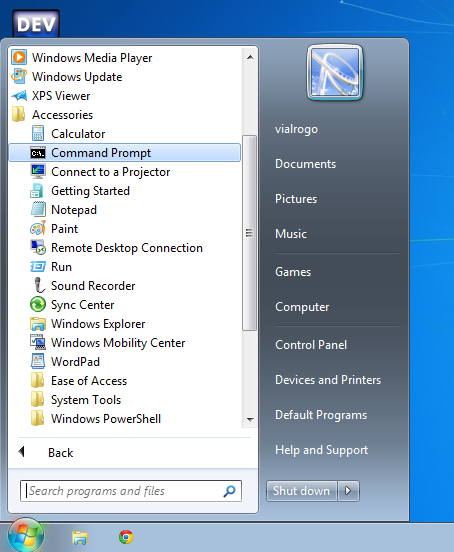
\includegraphics[width=90mm]{Imagens/2.png}
  \caption{Prompt de comando (interfase em inglês)}
\label{fig:2}
\end{figure}

No terminal usamos as instruções \emph{cd} e \emph{dir} para chegar no pasta na qual está nosso programa.
Depois podemos executar o programa simplesmente digitando seu nome e a continuação nossos parâmetros de entrada:

\begin{figure}[H]
  \centering
  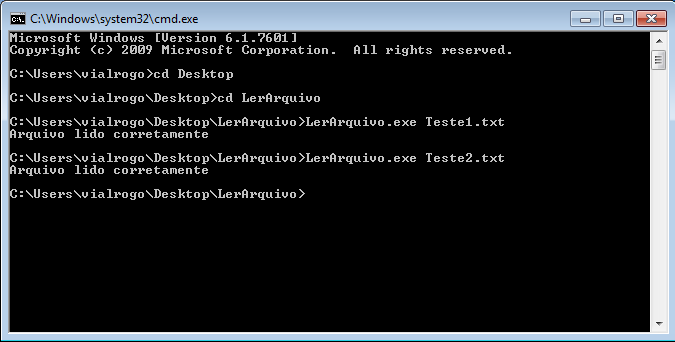
\includegraphics[width=140mm]{Imagens/1.png}
  \caption{Execução com parâmetros na linha de comando}
\label{fig:1}
\end{figure}

\subsection*{Configuração de DeC++ para o passo de argumentos}
Outra alternativa é configurar DevC++ para que passe parâmetros a nosso programa.
Para fazer isto vamos a \emph{Executar}, \emph{parâmetros}:

\begin{figure}[H]
  \centering
  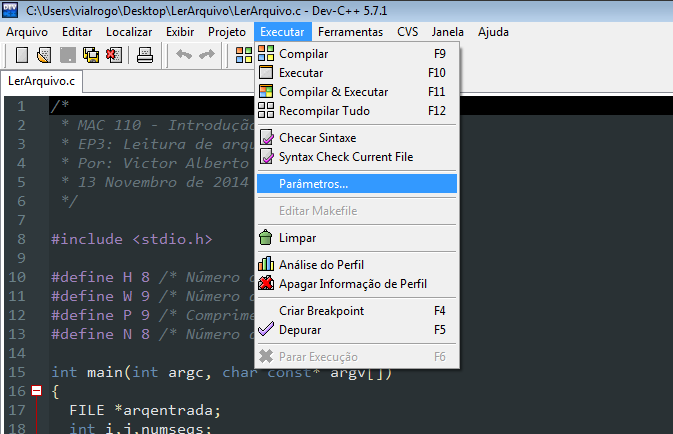
\includegraphics[width=140mm]{Imagens/3.png}
  \caption{Menu de Ferramentas}
\label{fig:3}
\end{figure}

No quadro que aparece a seguir agregamos os parâmetros de execução:

\begin{figure}[H]
  \centering
  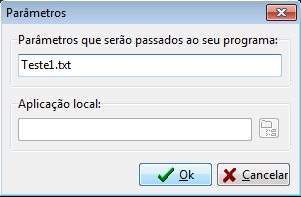
\includegraphics[width=80mm]{Imagens/4.png}
  \caption{Menu de Ferramentas}
\label{fig:4}
\end{figure}

Com isso, na próxima execução do programa vão se inserir os parâmetros.

\end{document}
